\section{Auswertung}
\label{sec:Auswertung}

\subsection{Kontrast}
\label{subsec:Kontrast}
Zu Beginn der Auswertung wurde der maximale Kontrast ermitttelt, der dann für die weitere Auswertung verwendet wurde.
Wie in der Durchführung \ref{subsec:Kontrastbestimmmung} beschrieben, wurden die Messpunkte aufgenommen und mithilfe von Gleichung \eqref{eqn:kontrast} wurde der Kontrast bestimmt.
Die Ergebnisse sind in \autoref{tab:Kontrast} zu finden.
Der maximale Kontrast mit $K = \num{0.97}$ wurde bei $\phi = \SI{135}{\degree}$ bestimmt.
Somit wurde der Polarisatiosfilter für die folgenden Messungen auf $\phi = \SI{135}{\degree}$ gestellt.

\noindent
Desweiteren wird mit den Messwerten eine Ausgleichsrechnung mit python durchgeführt.
Der Kontrast $K$ kann mit folgender Funktion beschrieben werden:
\begin{equation}
  K = A \cdot | \cos(\Phi)\sin(\Phi) | \, . \label{eqn:kontrast_rechnung}
\end{equation}
Durch die Ausgleichsrechnung wird für 
\begin{equation*}
  A = 1,89 \pm 0,05
\end{equation*} 
ermittelt.
Die aufgenommenen Messwerte, sowie die Ausgleichsfunktion sind in \autoref{fig:Kontrast_Ausgleich} grafisch abgebildet.

\begin{figure}[H]
  \centering
  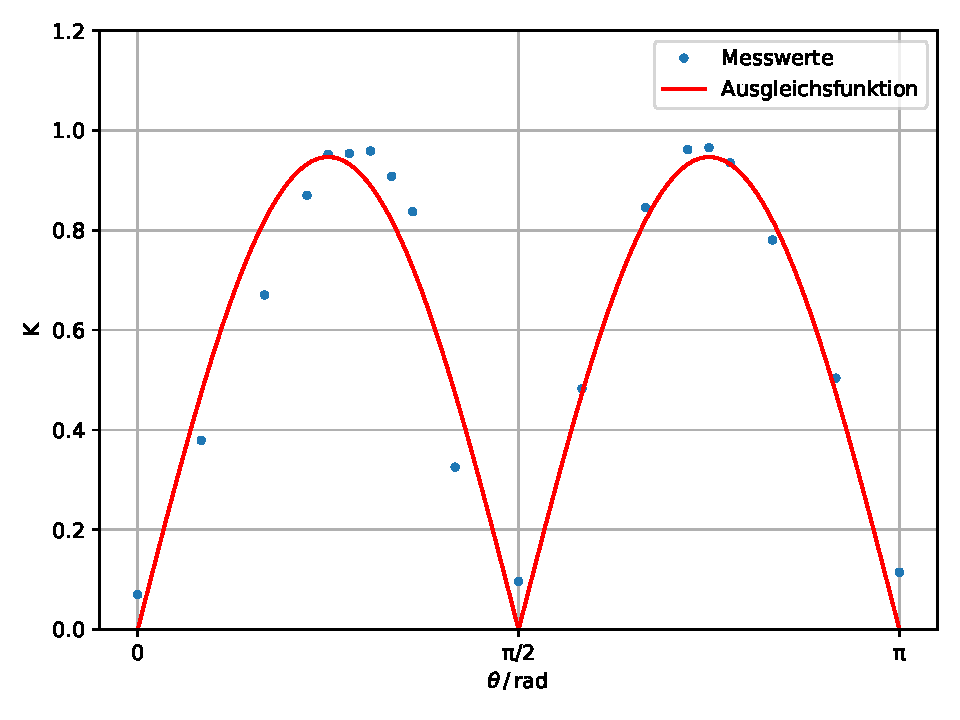
\includegraphics[width=\textwidth]{build/kontrast_ausgleich.pdf}
  \caption{Die Messwerte des Kontrast nach Gleichung \eqref{eqn:kontrast} und die Ausgleichsrechnung nach Gleichung \eqref{eqn:kontrast_rechnung}.}
  \label{fig:Kontrast_Ausgleich}
\end{figure}

\begin{table}[H]
  \centering
  \caption{Aufgenommene Messwerte zur Kontrastmessung, sowie der jeweilige Kontrastwert.}
  \label{tab:Kontrast}
  \begin{tabular}{c c c c}
    \toprule
    $\Phi / \si{\degree} $ & $U_{\text{min}} / \si{\volt}$ & $U_{\text{max}} / \si{\volt}$ & $K$ \\
    \midrule
    0     &  0,86  &  0,99  & 0,07  \\
    15    &  0,36  &  0,80  & 0,38  \\
    30    &  0,14  &  0,71  & 0,67  \\
    40    &  0,05  &  0,72  & 0,87  \\
    45    &  0,02  &  0,82  & 0,95  \\
    50    &  0,02  &  0,85  & 0,95  \\
    55    &  0,02  &  0,96  & 0,96  \\
    60    &  0,05  &  1,04  & 0,91  \\
    65    &  0,10  &  1,13  & 0,84  \\
    75    &  0,58  &  1,14  & 0,33  \\
    90    &  0,84  &  1,02  & 0,10  \\
    105   &  0,60  &  1,72  & 0,48  \\
    120   &  0,22  &  2,63  & 0,85  \\
    130   &  0,06  &  3,08  & 0,96  \\
    135   &  0,05  &  2,85  & 0,97  \\
    140   &  0,10  &  3,00  & 0,94  \\
    150   &  0,32  &  2,60  & 0,78  \\
    165   &  0,62  &  1,88  & 0,50  \\
    180   &  0,77  &  0,97  & 0,11  \\
    \bottomrule
  \end{tabular}
\end{table}

\subsection{Brechungsindex von Glas}
\label{subsec:n_Glas}
Um den Brechungsindex von Glas zu bestimmen, wurde die Anzahl der Intensitätsminima $M$, wie in der Druchführung \ref{subsec:n_glas_Durchführung} beschrieben, aufgenommen.
Mithilfe der Gleichung \eqref{eqn:n_Glas} wurde der Brechungsindex bestimmt.
Dabei beträgt die Dicke der Platten $D = \SI{1}{\milli\metre}$, die Wellenlänge des Lasers $\lambda_0 = \SI{632.990}{\nano\metre}$ und $\theta_0 = 10°$, da die beiden Platten jeweils um $\pm \theta_0$ geneigt waren \cite{anleitung}.
Die aufgenommenen Messwerte sowie der jeweils ermittelte Brechungsindex sind in \autoref{tab:Glas} zu finden.
Im Mittel beträgt der ermittelte Brechungsindex für Glas 
\begin{equation*}
    n_\text{Glas} = 1,55044793 \,.
\end{equation*}

\begin{table}[H]
  \centering
  \caption{Aufgenommene Messwerte zur Bestimmung des Brechungsindex von Glas, sowie der ermittelte Brechungsindex.}
  \label{tab:Glas}
  \begin{tabular}{c c c}
    \toprule
    Durchgang & M & $n_\text{Glas}$ \\
    \midrule
    1    &   30    &   1,45284966\\
    2    &   35    &   1,57145515\\   
    3    &   36    &   1,59753863\\   
    4    &   36    &   1,59753863\\   
    5    &   35    &   1,57145515\\   
    6    &   35    &   1,57145515\\   
    7    &   35    &   1,57145515\\   
    8    &   36    &   1,59753863\\   
    9    &   31    &   1,47511653\\   
    10   &   32    &   1,49807656\\   
    \bottomrule
  \end{tabular}
\end{table}

\subsection{Brechungsindex von Luft}
\label{subsec:n_Luft}
Zur Bestimmung des Brechungsindex von Luft wurden die Messwerte, wie in der Durchführung \ref{subsec:Durchführung_n_Luft} beschrieben, aufgenommen und 
die Brechungindices mithilfe der Gleichung \eqref{eqn:n_Luft} ermittelt.
Die Länge der Gaskammer beträgt $L = \SI[separate-uncertainty = true]{100(1)}{\milli\metre}$ \cite{anleitung} und die aufgenommene Temperatur $T = \SI{21.1}{\celsius}$.
Die aufgenommenen Messwerte sind in \autoref{tab:Luft} zu finden.
% Der durchschnittliche Brechungsindex für jeden Durchgang ist in \autoref{tab:n_luft_mean} aufgelistet.
% Für den durchschnittlichen Brechungsindex ohne Haube wurde
% \begin{equation*}
  % n_\text{Luft,ohne} = 1,0001703 \pm 0,0000017
% \end{equation*}
% und mit Haube 
% \begin{equation*}
  % n_\text{Luft,mit} =  1,0001622 \pm 0,0000016
% \end{equation*}
% gemessen.

\begin{table}[H]
  \centering
  \caption{Aufgenommene Messwerte zur Bestimmung des Brechungsindex von Luft neben dem jeweil nach Gleichung \eqref{eqn:n_Luft} errechneten Brechungsindex.
            $M_i$ bezeichnet hierbei die Anzahl der bis dahin durchlaufenden Interferenzminima oder -maxima, wobei $i$ den Durchgang angibt.}
  \label{tab:Luft}
  \begin{tabular}{c S[table-format=2.0] S[table-format=1.8] S[table-format=2.0] S[table-format=1.8] S[table-format=2.0] S[table-format=1.8] S[table-format=2.0] S[table-format=1.8]}
    \toprule
    & \multicolumn{4}{c}{Durchgänge ohne Haube} & \multicolumn{4}{c}{Durchgänge mit Haube} \\
    \cmidrule(lr){2-5} \cmidrule(lr){6-9} 
   {$p / \si{\milli\bar}$} & {$M_1$} & {$n_1$} & {$M_2$} & {$n_2$} & {$M_3$} & {$n_3$} & {$M_4$} & {$n_4$} \\
    \midrule
    50    &   4    & 1,00002532   &   5    & 1,00003165   &   2     & 1,00001266  &    2  &  1,00001266   \\
    100   &   6    & 1,00003798   &   7    & 1,00004431   &   4     & 1,00002532  &    4  &  1,00002532   \\
    150   &   8    & 1,00005064   &   10   & 1,00006330   &   7     & 1,00006330  &    10 &  1,00004431   \\
    200   &   10   & 1,00006330   &   12   & 1,00007596   &   9     & 1,00007596  &    12 &  1,00005697   \\
    250   &   12   & 1,00007596   &   14   & 1,00008862   &   11    & 1,00008862  &    14 &  1,00006963   \\
    300   &   14   & 1,00008862   &   16   & 1,00010128   &   13    & 1,00013293  &    21 &  1,00008229   \\
    350   &   17   & 1,00010761   &   18   & 1,00011394   &   15    & 1,00014559  &    23 &  1,00009495   \\
    400   &   20   & 1,00012660   &   20   & 1,00012660   &   17    & 1,00015825  &    25 &  1,00010761   \\
    450   &   23   & 1,00014559   &   22   & 1,00013926   &   19    & 1,00017091  &    27 &  1,00012027   \\
    500   &   25   & 1,00015825   &   24   & 1,00015192   &   21    & 1,00018357  &    29 &  1,00013293   \\
    550   &   28   & 1,00017724   &   26   & 1,00016458   &   24    & 1,00019623  &    31 &  1,00015192   \\
    600   &   32   & 1,00020256   &   29   & 1,00018357   &   26    & 1,00021522  &    34 &  1,00016458   \\
    650   &   36   & 1,00022788   &   31   & 1,00019623   &   28    & 1,00022788  &    36 &  1,00017724   \\
    700   &   39   & 1,00024687   &   33   & 1,00020889   &   30    & 1,00024054  &    38 &  1,00018990   \\
    750   &   42   & 1,00026586   &   35   & 1,00022155   &   32    & 1,00025320  &    40 &  1,00020256   \\
    800   &   44   & 1,00027852   &   37   & 1,00023421   &   34    & 1,00026586  &    42 &  1,00021522   \\
    850   &   47   & 1,00029751   &   39   & 1,00024687   &   36    & 1,00027852  &    44 &  1,00022788   \\
    900   &   50   & 1,00031650   &   41   & 1,00025953   &   38    & 1,00029118  &    46 &  1,00024054   \\
    950   &   54   & 1,00034181   &   43   & 1,00027219   &   41    & 1,00030384  &    48 &  1,00025953   \\
    1000  &   58   & 1,00036713   &   45   & 1,00028485   &   42    & 1,00031650  &    50 &  1,00026586   \\ 
    \bottomrule
  \end{tabular}
\end{table}

% \begin{table}[H]
%   \centering
%   \caption{Der durchschnittliche Brechungsindex von Luft für jeden Durchgang. Durchgang 1 und 2 wurden ohne Haube durchgeführt, Durchgang 3 und 4 mit.}
%   \label{tab:n_luft_mean}
%   \begin{tabular}{c c}
%     \toprule
%     Durchgang & $n_\text{Glas}$ \\
%     \midrule
%     1    &  $1,0001801 \pm 0,0000018$ \\   
%     2    &  $1,0001605 \pm 0,0000016$ \\   
%     3    &  $1,0001823 \pm 0,0000018$ \\   
%     4    &  $1,0001421 \pm 0,0000014$ \\   
%     \bottomrule
%   \end{tabular}
% \end{table}

\subsubsection{Lorentz-Lorenz Gesetz}
Da der Brechungsindex von Gasen nach dem Lorentz-Lorenz Gesetz auch vom Druck und  der Temperatur abhängig ist, wird nach Gleichung \eqref{eqn:Lorentz_Lorenz} eine Ausgleichsrechnung durchgeführt.
Die Ausgleichsfunktion hat dabei die Form
\begin{equation*}
  n = \frac{a}{TR} \cdot p + b \, .
\end{equation*}
Nach einer Temperaturmessung ergab sich für $T = \SI{21.1}{\celsius} = \SI{294.25}{\kelvin}$, $R$ beschreibt die universale Gaskonstante.
Die Ausgleichsrechnung wird für alle vier Durchgänge gemacht.
Für die Variablen $a$ und $b$ ergeben sich somit die Werte in der \autoref{tab:ausgleich}. 
\begin{table}[H]
  \centering
  \caption{Die Ergebnisse der Ausgleichsrechnung für die Variablen $a$ und $b$ je Durchgang. Durchgang 1 und 2 wurden ohne Haube durchgeführt, Durchgang 3 und 4 mit.}
  \label{tab:ausgleich} 
  \begin{tabular}{c c c}
    \toprule
    Messung & $a / \left(10^{-2} \si{\cubic\metre\per\mole} \right)$ & $b$ \\
    \midrule
    1    &  $0,00088982 \pm 0,00001704$ & $0,99998914 \pm 0,00000417$ \\   
    2    &  $0,00065089 \pm 0,00000369$ & $1,00002079 \pm 0,00000090$ \\   
    3    &  $0,00076337 \pm 0,00002429$ & $1,00001849 \pm 0,00000595$ \\   
    4    &  $0,00065508 \pm 0,00000415$ & $1,00000153 \pm 0,00000102$ \\
    \bottomrule
  \end{tabular}
\end{table}
\noindent
Die aus den Messwerten berechneten Brechungsindizes und die daraus ermittelten Ausgleichsgraden sind in \autoref{fig:lorentz_lorenz} zu finden.

\noindent Nach dem Lorentz-Lorenz-Gesetz wird für jeden Durchgang der Brechungsindex bei Normatmosphäre berechnet. Dabei ist 
$T = \SI{15}{\celsius} = \SI{288.15}{\kelvin}$ und $p = \SI{1013}{\milli\bar}$. Die Werte sind in der \autoref{tab:n_luft_mean}. 

\begin{table}[H]
  \centering
  \caption{Der Brechungsindex von Luft  bei Normatmosphäre für jeden Durchgang. Durchgang 1 und 2 wurden ohne Haube durchgeführt, Durchgang 3 und 4 mit.}
  \label{tab:n_luft_mean}
  \begin{tabular}{c c}
    \toprule
    Durchgang & $n_\text{Luft}$ \\
    \midrule
    1    &  $1,00036537 \pm 0,00000832$ \\   
    2    &  $1,00029600 \pm 0,00000180$ \\   
    3    &  $1,00034126 \pm 0,00001187$ \\   
    4    &  $1,00027852 \pm 0,00000203$ \\   
    \bottomrule
  \end{tabular}
\end{table}

\noindent Für den Brechungsindex bei Normatmosphäre ohne Haube wurde somit 
\begin{equation*}
  n_\text{Luft,ohne} = 1,000331 \pm 0,000004
\end{equation*}
und mit Haube 
\begin{equation*}
  n_\text{Luft,mit} = 1,000310 \pm 0,000006
\end{equation*}
ermittelt.\\
Im Durchschnitt haben die Fitparameter folgenden Wert:
\begin{align*}
  a = \SI{0.000740(8)e-2}{\cubic\metre\per\mole}& &b = 1,0000075 \pm 0,0000018
\end{align*}
Damit beträgt der durchschnittliche Brechungsindex von Luft mit diesen Werten und bei Normatmosphäre 
\begin{equation*}
  n_{\text{Luft}} = 1,000320 \pm 0,000004 \, .
\end{equation*}

\begin{figure}[H]
  \centering
  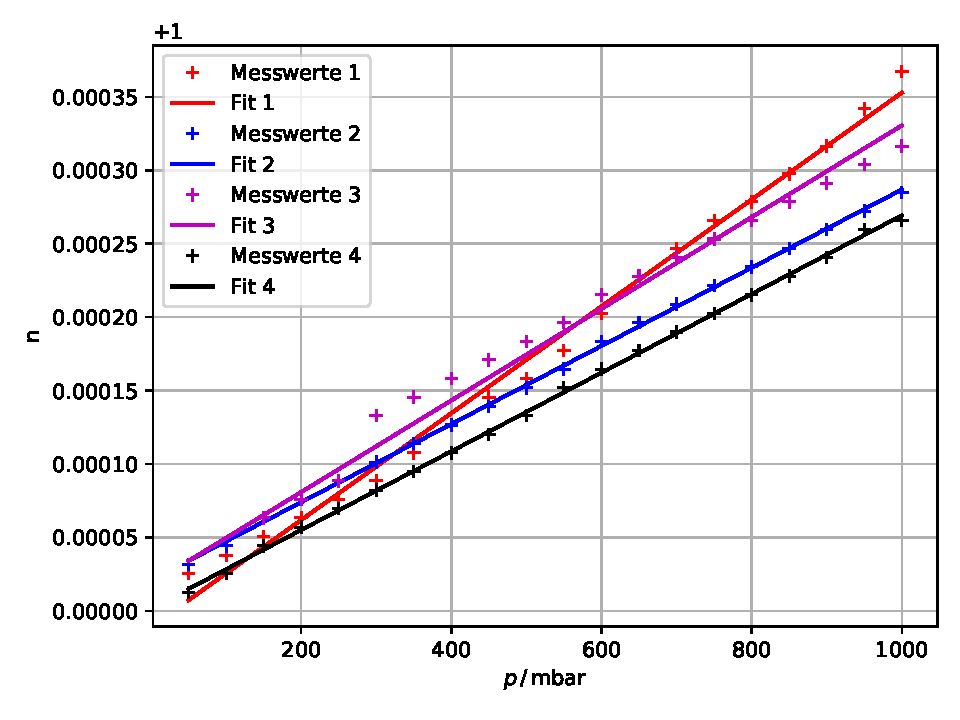
\includegraphics[width=\textwidth]{build/lorentz_lorenz.pdf}
  \caption{Die aus den aufgenommenen Messwerten bestimmten Brechungsindizes $n$ für Luft und die Ausgleichsgraden.
  Messung 1 und 2 wurden ohne Haube durchgeführt, Messung 3 und 4 mit.}
  \label{fig:lorentz_lorenz}
\end{figure}